
\documentclass{article}
\usepackage[nottoc,numbib]{tocbibind}
%\usepackage[nottoc]{tocbibind}
\usepackage{setspace}
\usepackage[utf8]{inputenc}
\usepackage[table,xcdraw]{xcolor}
\usepackage{listings}
\usepackage{multirow}
\usepackage{blindtext}
\usepackage{tikz}
\usepackage{float}
\usepackage{fontspec}
\usepackage[
	margin=1.5in,
	footskip=1.2in
	]{geometry}
\usepackage{fancyhdr}
\usepackage{mwe}
\usepackage{graphbox}
\pagestyle{fancy}
\usepackage{graphicx}
\usepackage[export]{adjustbox}
\usepackage{xcolor}
\lstset {
	breaklines=true
}
\usepackage{tocloft}
%JAMK custom color, used to print The Line
\definecolor{JamkBlue}{rgb}{0,90,125}
\renewcommand\cftsecleader{\cftdotfill{\cftdotsep}}

%Title page needs special attention: line in the left
\fancypagestyle{TitlePage}
{
	\fancyhf{}
	\renewcommand{\headrulewidth}{0pt}	
	\lhead{
		\begin{tabular}[t]{l@{\hspace{3cm}}l}	
		
\includegraphics[scale=0.22]{jamk-logo}
		\end{tabular}	
		}
	\newgeometry{left=4cm}	
	\cfoot{
\includegraphics[valign=B,scale=1.2]{jamk-footer} }	
}

%clear headers&footers
\fancyhf{}
\renewcommand{\headrulewidth}{0pt}
%insert jamk -footer logo to each page
%\cfoot{
\includegraphics[valign=B,scale=1.2]{jamk-footer} }
\setmainfont{Carlito-Regular}
\parskip = \baselineskip
\usepackage[parfill]{parskip}
 
\begin{document}
\onehalfspacing
\begin{titlepage}
\thispagestyle{TitlePage}
    \vfill
    \begin{tabular}[t]{l@{\hspace{0cm}}l}
     &
     \begin{tabular}[t]{p{0.85\textwidth}}
     \\ \\ \\ \\ \\ \\ \\ \\ \\ \\ \\ 
     \textbf{\Large {How to self-assess and audit application deployment in public cloud? }} \\ [2cm]
	\large{Pinja Koskinen} \\	
	\large{Vesa Simola} \\
       { \date{ } }  
	\\ \\ \\ \\ \\ \\ \\ \\ \\
	\large{Masters thesis}\\
	\large{XXXXX 2018}\\
	\large{Cyber security}\\
	\large{Master's degree programme in cyber security}
	\end{tabular}
    \end{tabular}

\end{titlepage}

\clearpage 
\begin{table}[]
\centering
\label{my-label}
\begin{tabular}{|l|l|l|}
\hline
\multirow{3}{*}{\begin{tabular}[c]{@{}l@{}}Author(s)\\ Pinja Koskinen, Simola, Vesa\end{tabular}} & \multirow{2}{*}{\begin{tabular}[c]{@{}l@{}}Type of publication\\ Masters thesis\end{tabular}} & \begin{tabular}[c]{@{}l@{}}Date\\ Month Year\end{tabular}                  \\ \cline{3-3} 
                                                                                        &                                                                                                & \begin{tabular}[c]{@{}l@{}}Language of publication:\\ English\end{tabular} \\ \cline{2-3} 
                                                                                       & Number of pages                                                                                & Permission for web publication: x                                          \\ \hline
\multicolumn{3}{|l|}{\begin{tabular}[c]{@{}l@{}}Title of publication\\ Title\\ possible subtitle\end{tabular}}                                                                                                                                                       \\ \hline
\multicolumn{3}{|l|}{Degree programme}                                                                                                                                                                                                                                \\ \hline
\multicolumn{3}{|l|}{\begin{tabular}[c]{@{}l@{}}Supervisor(s)\\ Last name, First name\end{tabular}}                                                                                                                                                                  \\ \hline
\multicolumn{3}{|l|}{Assigned by}                                                                                                                                                                                                                                    \\ \hline
\multicolumn{3}{|l|}{\multirow{5}{*}{Abstract}}                                                                                                                                                                                                                      \\
\multicolumn{3}{|l|}{}                                                                                                                                                                                                                                               \\
\multicolumn{3}{|l|}{}                                                                                                                                                                                                                                               \\
\multicolumn{3}{|l|}{}                                                                                                                                                                                                                                               \\
\multicolumn{3}{|l|}{}                                                                                                                                                                                                                                               \\ \hline
\end{tabular}
\end{table}
\clearpage

\doublespacing
\tableofcontents
%Insert page number to right upper corner (header)
\pagebreak 
\setcounter{page}{1}
\rhead{\thepage}
\section{Introduction}
This thesis is about coming up with the self-assessment and auditing mechanism for Finnish applications that are either already deployed in public cloud or for applications that are candidates for such deployments. By being seen as flexible, reliable and cost effective mean of application delivery it is no wonder that the usage of cloud computing has spread far and wide.
Yet, there are usecases where public cloud platforms might not be optimal, feasible or, in some cases, allowed options for deployment. This paper was written to better understand the implications of cloud computing versus the requirements of certain official security, confidentiality, integrity and availability requirements, some of which are actual hard requirements set by Finnish officials and some that are more like recommendations and best practices. To make the matter even more complex there are several providers who sell public cloud. For the most part, the goods being offered are fairly similar in fashion or at least they provide the same basic building block upon to build ones application. Still, there are differences that could effect on the audit result that determines whether the particular application is a good candidate for cloud deployment, one example of such difference could be the various connectivity options for attaching the users to the cloud application, another example could be the layers provided by the services provider for building the defence in depth setting that is seen as a good practice. These small, but important variations may have dire consequences concerning the confidentiality, integrity or availability of the application and hence they need to be evaluated when determining if the application is a good candidate for cloud deployment at all and what provider or providers to select for the actual application deployment.
\par
This thesis starts by building up the basis of what is cloud computing and what it is made of, what kind of different cloud service categories are available currently and we'll also discuss some of the deployment models of cloud computing. Some emphasis is also put on the application design required to better exploit the possibilities of cloud by means of using stateless micro services with containers and orchestration tools. Security aspects of each of the factors and what they bring into the table are considered from the classical CIA-perspective, eg. Confidentiality, Integrity and Availability. Last portions of this thesis consist of the self-assessment questionaire and the audit criteria. These two can be used to assess application for cloud deployment and on the other hand to audit already existing application.
\par
Last parts of this text will concentrate on assessing and auditing application deployment in cloud based on the topics discussed before. The self assessment questionaire and audit procedure are hopefulle helpfull when determining if particular application is suitable for deployment in public cloud.
\section{General overview of cloud services}
Cloud service is generally understood as a product consisting of outsourced IT infrastructure, software components and some means for the customer to manage the service. This results in scalable distributed compute resources that are accessed using the network where several factors like CPU, memory and storage can be adjusted according to current needs (Hausman, Kirk, Susan L. Cook, and Telmo Sampaio. "Chapter 1 - What is Cloud Computing?". Cloud Essentials: CompTIA Authorized Courseware for Exam CLO-001. Sybex. 2013. Books24x7. <http://common.books24x7.com.ezproxy.jamk.fi:2048/toc.aspx?bookid=52677> (accessed September 25, 2018) ). Also, cloud services tend to have scalability built-in in terms of having some for of pay-as-you-grow model, meaning that the customer can start off some amount of capacity but increase the deployment size as their requirements change, same is true for down scaling the capacity to avoid unused capacity overhead.
Avoiding costs is seen as one of the major benefits of cloud computing as many of the costly bits and bobs of IT infrastructure and related personnel can in many cases be outsourced. This means things including, but not limited to:
\begin{description}
	\item[$\bullet$ Datacenter facilities]
	\item[$\bullet$ Electricity, cooling etc.]
	\item[$\bullet$ Computer hardware]
	\item[$\bullet$ Operating systems to run on the hardware]
	\item[$\bullet$ Storage systems]
	\item[$\bullet$ Internet facing connectivity]
\end{description}
This makes cloud computing seem like an ideal option for certain use cases where company has no interest of hosting the infrastructure on their own. Instead of maintaining the above mentioned infrastructure, company can concentrate on they key business be it application development or the sales generated from their Internet shop. This is not always the case though, as we've discovered in later parts of this thesis.
\subsection{Cloud terminology and concepts}
Next we'll cover some of the generic concepts and basic terminology involved in cloud computing.
At the time of writing the cloud services can be split into three rough main categories (What is cloud computing Microsoft Azure 2018), and we'll discuss each of the aforementioned categories separately bellow. It should be noted that the categories below are subject to change as the cloud computing evolves and also there will likely be overlap in real life scenarios. Example of such overlap could be PaaS service providing Kubernetes workflow automation while at the same time Kubernetes itself could be seen as a SaaS service.
This overlap is natural result of the categories building on top of each other.
We'll also touch the few options for hosting the the cloud, either as a completely outsourced service, inhouse and the mixture of the two.
Security and availability aspects of the categories and their hosting options are discussed in detail later in this document. 
\subsubsection{Infrastructure-as-a-service, IaaS}
This is the basic service where one rents computing capacity in a form of facilities that house hardware, virtual machines, storage capacity and network bandwidth.
Operating systems and some core infrastructure services such as NFS storage or firewalls could be provided as part of the service. This category of cloud computing provides the basic pay-as-you-grow model in terms of giving the customer the opportunity to scale their number of virtual machines, storage capacity or pretty much any of the basic building blocks.
The benefit of the IaaS cloud for the customer is that certain data center related activities can be abstracted and used from for example a web interface or an API. There is no need to manage all levels of the infrastructure anymore and administative tasks can mostly focus on server side level like operating systems management and maintenance, and third party software maintenance. (Kavis, Michael. "Infrastructure as a Service". Architecting the Cloud: Design Decisions for Cloud Computing Service Models (SaaS, PaaS, and IaaS). John Wiley \& Sons. 2014. Books24x7. <http://common.books24x7.com.ezproxy.jamk.fi:2048/toc.aspx?bookid=62597> (accessed September 25, 2018), Infrastructure as a Service )
As in this type of a cloud service only the infrastructure is provided, all software related development and administration responsibilities are left to the customer (Kavis, Michael. "Infrastructure as a Service". Architecting the Cloud: Design Decisions for Cloud Computing Service Models (SaaS, PaaS, and IaaS). John Wiley \& Sons. © 2014. Books24x7. <http://common.books24x7.com.ezproxy.jamk.fi:2048/toc.aspx?bookid=62597> (accessed September 25, 2018), Infrastructure as a Service ). While this brings a lot of freedom on how to create the software and configuration, nothing is provided as a service by the cloud provider.
It should also be noted that while service provider can have multiple geographical sites from which they provide their service allowing distribution of the resources, none of this is benefitting the software stack without adding additional features to the software. To benefit from this the cloud awareness and scalability has to be done either manually or as a part of the software. Some of these limitations and distribution of responsibilities are discussed next.
\newpage
Given that part of the infrastructure is being outsourced to external service provider it is essential to understand the implications to responsibilities this approach brings with it. Also, different failure domains play important role in assessing the feasibility of the IaaS deployment.
Picture below tries to identify some of the minium responsibility zones this IaaS creates.
\begin{figure}
    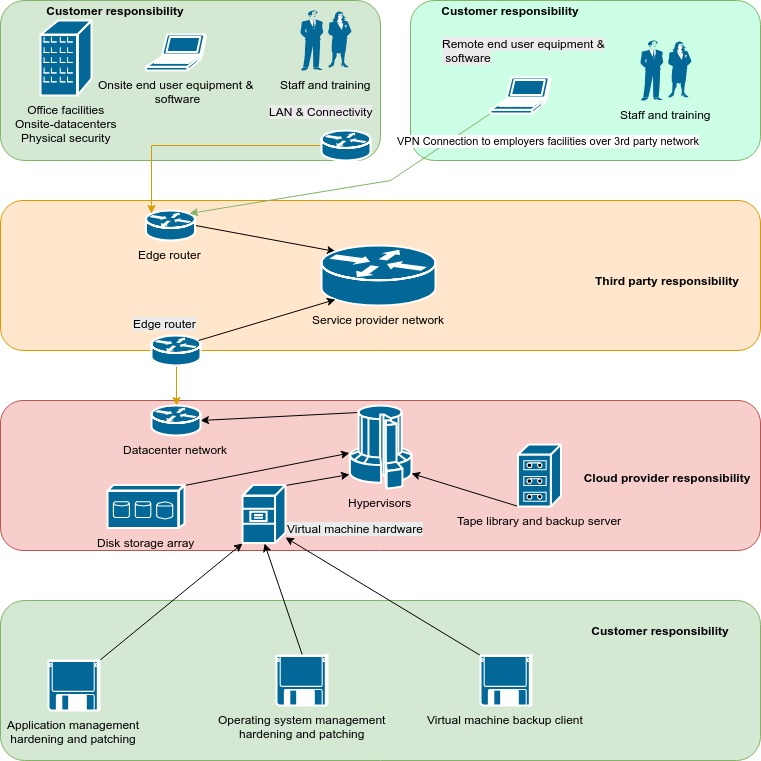
\includegraphics[width=10cm,height=10cm]{thesis_iaas.jpg}
    \caption{Iaas Architechture and responsibility zones}
    \label{Figure:IaaS architechture}
\end{figure}
\subsubsection{Platform-as-a-service, PaaS}
As stated above IaaS does not address the many of the scalability issues or automation challenges faced by organizations especially from the perspective of a software. All the parts of the software infrastructure must be provided by the customer. To ease this task PaaS providers can provide software platforms to certain level. Typical software platforms can be for example databases, logging and payments services, which can be used via various APIs (Kavis, Michael. "Platform as a Service". Architecting the Cloud: Design Decisions for Cloud Computing Service Models (SaaS, PaaS, and IaaS). John Wiley \& Sons. © 2014. Books24x7. <http://common.books24x7.com.ezproxy.jamk.fi:2048/toc.aspx?bookid=62597> (accessed September 25, 2018) )
Several PaaS related technologies also aim at automating the provisioning procedures for the virtual machines and containers that actually run the application. Examples of these services could be for example a Kubernetes platform, which would provide an API for containers for automatic scalability. Containers are relatively new concept in computing but they are used to package the application and its dependencies in to a manageable units for distribution and running in cloud platform. (What is a container? Docker documentation 2018). These containers can then be housed in orchestration tools such as the aforementioned Kubernetes or Docker swarm. 
Usually PaaS service includes the IaaS services as well, but this is not a given. Many big cloud providers like AWS provide tend to provide a variety of platforms in addition to the plain infrastructure to meet different needs.
\subsubsection{Software-as-a-service, SaaS}
Software as a service is a method of delivering software application from cloud via Internet connectivity with the least amount of manual work from customer. Using SaaS only requires configuration and user management from the customer, leaving everything else for the service provider. The advantages to the customer is the lack of need to maintain the platform and not needing any personnel to execute the maintenance tasks, which is beneficial especially when talking about services that do not belong to the core functionalities of the customer. (Kavis, Michael. "Software as a Service". Architecting the Cloud: Design Decisions for Cloud Computing Service Models (SaaS, PaaS, and IaaS). John Wiley \& Sons. © 2014. Books24x7. <http://common.books24x7.com.ezproxy.jamk.fi:2048/toc.aspx?bookid=62597> (accessed September 25, 2018) ) Naturally, the SaaS services can not be used for software that require any heavier tayloring than just predefined configuration changes.
A real-life example that illustrates the stacking of cloud services and the SaaS could be a email service that has its customer specific frontends running in containers on service provider orchestration tool that utilizes virtual machines housed in service provider facilities and hypervisors somewhere. SaaS services are nowadays very common (Kavis, Michael. "Software as a Service". Architecting the Cloud: Design Decisions for Cloud Computing Service Models (SaaS, PaaS, and IaaS). John Wiley \& Sons. © 2014. Books24x7. <http://common.books24x7.com.ezproxy.jamk.fi:2048/toc.aspx?bookid=62597> (accessed September 25, 2018)).
\subsubsection{Differences between public and private cloud}
There are two different approaches to the clouud deployment in general, private cloud and public cloud. With private cloud the data and services are hosted hardware dedicated to particular end user organization, while public cloud shares the same hardware infrastructure across all the tenants. This is important aspect to understand when planning application deployment to cloud environment as private cloud provides few key security enhancements per default while at the same time some of the main benefits of cloud deminish:
\begin{description}
	\item[$\bullet$ CPU and memory is dedicated so computational performance likely more predictable]
	\item[$\bullet$ Storage performance is easier to predict in terms of IOPS and especially latency]
	\item[$\bullet$ Vulnerabilities such as recent spectre and meltdown are limited to within one organization]
	\item[$\bullet$ Network capacity is easier to predict and it is possible to have less latency if housed locally]
	\item[$\bullet$ In some cases, privately housed and managed cloud might be more likely to pass audit for handling classified information]
\end{description}
First three of the above are fairly obvious, but the notion about using privately housed and managed cloud for audit compliance is worth of few further clarification. Finnish ministry of finance states in the VAHTI that when using shared capacity the organization is leaving the management and control of the platform to service provider. This highlights the  importance for the client organization to have efficient methods and processes for overseeing the service provider and to understand the nature of the information stored in the cloud and to have efficient means of confirming that the service provider acts according to the requirements and contracts. (VAHTIohje, vaatimukset tekniselle tietotekniikkaympäristölle, 2016). This could also be understood so that it is quite possible to run classified application in private cloud and gain all the provisioning benefits, as long as the environment supports the required security controls, management processes and that there are otherwise sustainable technical environment to run the application on. This is true regardless if the private cloud is hosted inside the customer company or physically from service provider facility.
\par
Public cloud on the other hand is generally purely shared capacity housed in service provider facilities and usually boasts all the outsourcing benefits within the cloud offering. While some public cloud offerings may have dedicated capacity, it is more often built around the performance factor. Example of this kind of performance oriented offering could be fatnodes with large amounts of RAM or GPU-computation capacity that is rented on hourly basis. That being said, public cloud can provide additional security features that can compensate for the shared infrastructure, like:
\begin{description}
	\item[$\bullet$ Data encryption at rest as given, with custom encryption keys]
	\item[$\bullet$ Multifactor authentication to cloud management portal]
	\item[$\bullet$ Redundant connectivity from service provider facilities]
\end{description}
It goes without saying that the list above is not by no means complete and that all of the above are possible to implement in private cloud as well.
\subsubsection{Mixtures of the two, aka hybrid cloud}
For some implementations it would be ideal to combine the two, private and public cloud. Example of this type of deployment might be an application that has a Internet facing frontend running in service provider cloud, utilizing load balancers and firewalls offered as part of the cloud offering, while the database portion of the application is housed inside the customer datacenter, in customer hardware. Many vendors boast connectivity services that allow the "stretching" of in-house datacenter to service provider facilities. While flexible, this also creates complexity as it is more difficult to understand the dependencies of applications deployed in this manner. Also, it is worth noting that interconnecting data centers is quite complex topic on its own, especially if workloads are to be moved between locations. Some of the risks and implementation models are discussed in the later chapters.
\section{Security in cloud}
Security in cloud has several characteristics compared to traditional server infrastracture, especially in public and community cloud infrastructure. Private cloud mostly follows the traditional threat scenarios, nevertheless some aspects can be seen even here. In this chapter, we will cover several problems we have seen in cloud environments.
\subsection{Security in private cloud}
- Trusted environment
- Self hosted, or hosted by a trusted partner
The biggest difference between traditional server environments or even most of the virtual machine environments is the freedom often provided by the cloud environment. Thus users with less security awareness may be creating and maintaining instances, which may lead to poorer quality of servers in terms of security, a good example is servers meant for testing purposes. Also, if creating servers is more free across the personnel, this might lead to vague responsibilities and neglect of maintenance standards. An organisation has several means to mitigate these problems, for example by prividing custom images providing a certain level of security, by running security scans against the servers or by training to name a few examples.
(Todo: Generic stuff about backups and their role in security. )For recovery purposes the cloud environments don't necessarily provide decent native backup solutions. This used to be the case for example with OpenStack's earlier version. This easily lead to situations, where backups were easily neglected. Thus if there is a data loss by technical failure or as a result of a system breach, bringing up the system could be quite troublesome.
\subsection{Security in community cloud}
- Partly trusted
- Self hosted or hosted by a trusted or known partner
\subsection{Security in public cloud}
- Hosted by a known or unknown vendor
- You can not normally audit the vendor -> blindness
- Server location might change (take Apple's China incident) especially if vendor is an international actor
- Contract
- Mitigations
\subsection{Introduction to security aspects in cloud}
\subsection{Security aspects of application development in public cloud}
- Make application too fast for attackers (cloud native)
- The application can be provided from distributed location, same applies to data (which could be broken into meaningless pieces to fight data theft)
- Possibilities?
\subsection{Introduction to cloud security and application deployment}
\subsubsection{Source code control in cloud application development}
\subsubsection{Secure processes for updating application and library code}
\subsubsection{Secure application administration procedures}
- Best practices
- Limitation created by cloud environment
- Connections over internet
\subsection{Security and availability, and what to prepare for}
Players in the cloud service provider field tend to the well connected to Internet and to each other (FICIX,2018). This on its own gives service providers some edge when compared to inhouse data center and the connectivity options available. It is also fairly safe to assume that service providers also have more personnel available to run their infrastructure compared to small or medium size company whose business is non-IT-infrastructure.
\par
That being said, especially public cloud hosting with containers should not be seen as a similar virtualization platform as privately maintained in-house datacenter. There are numerous examples of cloud failures that could have been mitigated by understanding the nature of cloud computing and by building the application accordingly, e.g built-in distribution of application resources. Let us next review few of these incidents and discuss some of the remedies that could prevent or lessen the damage caused by these kind of incidents.
\subsubsection{File sharing service had authentication bug}
On June 2011 well known file sharing service faced an issue where some users could login to accounts without using correct password (dropbox,2011). This led to a situation where the files owned by these accounts were possibly exposed. According to the file sharing service they reacted to this issue by "ending all logged sessions". So not only was there a possibility of information leak, but also innocent users were kicked out of the system to safe guard the data, while the initial step of kicking out users in this sort of situation is not all that dramatic. But what could users do to avoid being denied access to their data, and on the other hand, how to protect their files stored in public cloud?
\par
First option would be to upload only encrypted files, this more or less solves the initial issue of data exposure given that reasonably strong encryption is used. The second threat of being left without access to files due to being kicked out of the service could be avoided by using multiple file sharing services, each with identical data. Now, this might sound laboursome but by using programmatic approach to upload files this replication work could be hidden from the end user. Similarly, downloading files could be done programatically hiding the underlying issue with one of the file sharing services. This programmatic approach would also lend itself nicely for the encryption as key handling could be automated to some extent as well. 
\subsubsection{Outsourced datacenter}
To discuss the merits and disadvantages of outsourced data center it is essential to define the meaning of outsourcing in the context of cloud services and data centers. Outsourcing is usually understood as improving the efficiency of business by transferring parts of work that are not seen as the core business to 3rd parties who specialize in those particular tasks, such as power distribution, cabling, IP and ethernet connectivity, rack installations, physical access control etc. (datacenterjournal.com, 2012)
Grand idea of outsourcing being that the 3rd party would have better set of skills to do the work in more efficient and reliable manner and possibly by means of volume do it cheaper too. In our context this could mean that company does not see running its own data center and all its dependencies as a core business element, instead company wants to focus on application development and selling application support and maintenance without too many regulations set by authorities or customers. This kind of requirements create decent starting point for investigating if particular application or set of applications could run in outsourced data center, possibly in cloud fashion. 
\subsubsection{Outsourced server etc. infrastructure, either partially or wholly}
As previously stated, there are few levels when it comes to outsourcing. Namely in our context this means either outsourcing all of the infrastructure required to run the application or parts of it. There could be situations where customer has enough resources to run their own servers and networking setup but they might lack the expertise required to maintain storage hardware or HPC connectivity.
These kind of mixtures of both outsourced and inhoused platforms require care and good communication with the service provider. As the responsibility is split between customer and the services provider it means that the fluent communication and processes are key as this is especially the case during troubleshooting or when deploying or planning changes to the environment that will require coordination. This is to avoid blamestorming in case something unexpected happens or when capacity expansions and scaling are required in timely fashion.
\subsubsection{Large cloud providers are certified, are they?}
\subsubsection{Cloud native applications: Maximize the benefits of cloud to protect data and services}
Although cloud environments can introduce several risks, they also provide an opportunity to improve the security. Several ideas are introduced in this section. Cloud has the advantage of being versatile, agile and distributed. These features can be used even in the well-known technologies.
\par
Cloud native applications are services, which are specifically build to recognize the surrounding provided by the cloud <todo: find a proper description>. The application can adjust to things like load and location. One idea of fighting attacks with cloud native solutions is provided by Nane Kratzke. With for example open source technologies like Kubernetes or Docker Swarm an environment that would move fast in case an attack is noticed could be made. An example solution could be a container based application, on top of virtual machines that could be in geographically disperse clouds and from different cloud providers. In case there is an attack directed at the platform, the containers could be moved to another environment, for example to another service provider before an attacker can gain a foothold at the environment. According to the paper, there are no known approaches to use this technology for security based solutions (About being the Tortoise or the Hare? A Position Paper on Making Cloud Applications too Fast and Furious for Attackers. Nane Kratzke, 2018. https://arxiv.org/pdf/1802.03565.pdf. Read 18.4.2018 <todo: check the date>). 
\par
Nevertheless, as availability is considered one aspects of security, this technique is well-known to provide this. To be used in the general context of security, there are some issues with this approach, as it is often hard to recognize underlying attacks. This we believe could be acquired at least to some extend with other traditional tehcnologies like SIEM, log analyzing and bug reports to name a few.
\subsubsection{Ready-to-deploy security improvements in cloud}
In addition to improving security on application level, it is possible to add to this goal with a hardened cloud platform. The big cloud providers like for example Amazon, Microsoft and Google do provide an extensive lists of measures to improve the security. Mostly these are provided by available security related products. To better understand what products these providers are seeing important, we'll introduce the tools these are providing. Monitoring is provided in different forms. For example Azure has a Azure Security Center, which provides views to different aspects of the cloud. Encryption is a common service to provide for all data, but there are big differences in key management, as in Amazon AWS it is possible to bring your own HMS device to improve the encryptions' security. It is also common to provide DDoS protection, providing this can be naturally also a benefit to the cloud provider itself, as as a multi user environment they are definitely targetted frequently through their customer base. Lastly identity management solutions are provided as an asset to ensure secure authentication and authorization. In addition to these examples, every one of these three providers have several other products, which seem to also derive their target customers from others. (AWS: https://aws.amazon.com/products/security/, https://docs.microsoft.com/en-us/azure/security/, https://cloud.google.com/security/products/)
\par
Sometimes it is possible to affect to the cloud installation, and in this case it becomes possible to create specific hardenings on the infrastructure's configuration. The individual components can be made more secure with additional configuration. It is also possible to add certain services like logging and monitoring, hardened base images, secure network configuration and also by auditing the systems security to name a few examples. From open source cloud platform software providers at least OpenStack  provides guides for ensuring the security of the installation (https://docs.openstack.org/security-guide/). As security is not just about technology, the administrative procedures and processes can be fine tuned to mitigate many risks.
\par
Even though a customer can add a lot to improve the security, there is only limited data available on how the public cloud providers ensure security in operations. The providers might have an extensive list of compliances like (https://cloud.google.com/security/compliance/, AWS artifact), but it is unlikely that even a mid-sized actor could make a proper audit for understandable reasons. Also the role of the service provider doesn't necessarily fit into the criteria's requirement, as the data owner is still the customer and not the provider. This can make a requirement and its fulfillment even vague. Also things like comprehensive and verbose audit reports from the existing are not available, so there is no data from for example restrictions done during the audit if there is a will to rely on existing audits.
\subsection{Security and availability cons of cloud deployments}
Security tends to be one of the largest concerns when when it comes to cloud computing and this is easy to understand as outsourced data center with cloud computing almost always exposes clients IT systems to third party such as service provider. (Data center journal, 2012). As discussed in the connectivity depency chapter, it is essential to have working connectivity to the application from campus, or if the application is solely dependant to Internet it should redundant access from the service provider facilities. While particular the service provider might be certified against ISO 27001 for example, it is still essential to have means of control for the impacts of data center outsourcing, this is especially true if ones application or service has to pass an audit from regulatory officials. To summarize the following cons can be identified:
\begin{description}
	\item[$\bullet$ Exposure of infrastructure to 3rd party]
	\item[$\bullet$ Importance of reliable Internet or WAN connectivity]
	\item[$\bullet$ Requires additional control for 3rd party if subject to regulation]
\end{description}
\subsubsection{Privacy implications of running application in cloud}
\subsubsection{Dependant to external 3rd party provider}
\subsubsection{Dependency to connectivity}
Since application is running the remote location it is obvious that connectivity is of paramount importance, in essense, having no connectivity in the campus means having no application and this can mean having no business. While many organizations have Internet connectivity these days it is still surprisingly uncommon for organizations to have backup connectivity if the unthinkable cut happens. Fiber cuts are not all that uncommon (Teddy Hayford-Acquah and Ben Asante, 2017) and while carrier backbone networks data center connections tend to be redundant in design, the so called "last mile" connection from service provider point-of-presence to customer can be a single point of failure. These non-redundant links can cause catastrophic failures when cut happens during business hours. There are couple of approaches to mitigate the availability issue presented by these failures as disscussed next.
\par
To reduce the impact of last mile failure it is common practice to have two physically separate lines from service provider, terminated to two separate customer premisses routers in two separate equipment rooms. (Gunnar Bøe, Vidar Faltinsen, Einar Lillebrygfjeld, 2011) Two routers using VRRP protocol act in active-passive manner to provide so-called first-hop redundancy (rfc5798, 2010). This approach, when combined with physically separate lines, provides protection from fiber cuts on the last mile and this also protects from power supply failures in the customer premisses router and also acts as a backup connection during router software upgrades and some configuration changes.
However, this method does not protect against catastrophic failures in the service provider network. To accomplish this, it is required to have similarly separated lines and routers from two separate service providers. Assuming that the customer has some IP block(s) to announce over BGP and that the service providers are accepting the customer IP block(s) for transit it is possible to create fully redundant last mile connectivity. All these relatively complex and expensive requirements are likely the reason why organizations wont purchase redundant connectivity but instead accept the risk of significant business impact and downtime. (Packetworks, 2016).
\par
Similarly, if cloud application is running in a "stretched" network infrastructure, eg. data center interconnect, it is essential that the interconnect is built in redundant fashion. While redundancy is all good it can also cause failures of different kind, but with equally potential for catastrophy (Pepelnjak, 2011) as we'll discuss next. 
\par
As most of the applications - in cloud, or otherwise - rely on IP connectivity it is unfortunate misconception that the underlying connectivity from two or more data centers and between datacenters is a given and identical. Having separate IP networks in data centers means that the server, container or whatever running the application looses its connectivity during workload transfer without reconfiguration of IP address and possibly DNS. Classic solution is to leave out the IP from the equation and simply strech the OSI layer 2 ethernet via means of OSI layer 1 technology to two or more datacenters. Given the broadcast nature of ethernet and how it behaves during loops this could be seen as a simple but dangerous approach that effectively stretches the data center but at the same time creates a large failure domain, eg. the feat of fate sharing if one data center has a loop the other one goes down as well. This is especially bad for applications that rely on OSI layer 2 signalling, such as redundant routers and firewalls (Pepelnjak, 2011). This problem with location redundancy could be solved by making the application layer not so reliant on the underlying IP layer, this could be done for example by decoupling the service IP - address that end users connect to - and advertising it to data center routers via BGP over only locally significant subnet. Even while there are tools for this sort of decoupling (RIPE 2010), this kind of approaches have apparently been deemed as non-trivial and time consuming tasks so currently it would appear that the accepted solution is to introduce more complexity outside the application to hide the underlying already existing complexity of IP transport. One such method is overlay networking, such as VXLAN, that builds up a streched OSI layer 2 domain over routed network (rfc7348).
\par
Above has been all about IP applications, yet majority of classical applications require storage to function. This means that storage has to be mirrored or replicated as well. As application generates value of some kind and it needs to store this newly created value somewhere this tends to mean that storage simply has to work. This is one of the reasons that still keeps fibre channel protocol alive, even while ethernet has gained whole load of new features that bring it closer to par with fibre channel when it comes to acting as a transport for storage traffic, eg. lossless connectivity via flow control and in-order-delivery. (Cisco, 2010 and Alex Grossman). Be that as it may, even FCoE still retains the fibre channel provisioning concepts such as zoning, masking and aliases and it is very much OSI layer 2 technology, similarly to native fibre channel. Traditional fibre channel implementations has two, physically and logically separated fabrics to guard against both hardware failures and misconfigurations. (Brocade, 2001). This is could be seen as a overkill these days, but when it comes to safeguarding ones most critical assets of an organization and what has been seen in the wild by the authors, this design still holds truth. Obviously, fibre channel supports streching of fabrics over geographical distances in highly available manner, within the latency window, but when it comes to virtualizing multiple tenants into physical fibre channel fabric the amount of scaling is limited (Brocade, 2015). This makes it non trivial for service providers to provide adequately separated, multi tenant storage connectivity from shared infrastructure. Hence, it is likely that if ones application deployment in private cloud relies on service provider facilities to provide on par redundancy for storage replication price tag might be signifficant. Fibre channel on public cloud is not an option.
\par
Another class of connectivity worth mentioning is the interprocess communication(IPC) and remote direct memory access (RDMA) protocols seen in high performance computing. These applications are very sensitive to latency to begin with and this makes these protocols less likely candidates for stretched fabrics. It should be also noted that protocols such as Infiniband are suited to carry IP and storage traffic in addition to their more commonly seen HPC traffic patterns. Yet, similarly to fibre channel infiniband has limited scalability in terms of multitenancy via number of tenant specific partitions available in the infiniband fabric (Mellanox, 2014). These protocols, just like fibre channel, are non trivial to stretch over large distances in feasible and multitenant manner.
\par
Regardless of the protocol being transported from end user to data center there is likely a need for encrypting the data while in transit. One approach is to implement the required encryption in the application itself by utilising TLS. It has been seen that to avoid complexity in applications there is a push to implement the encryption in the connectivity layer. While there are quite a few methods of implementing encryption in network it should be questioned if it is a sustainable choice to outsource application security to network layer. Implementing encryption using IPSEC (rfc4301) commonly indicates that OSI layer 3 routing should be implemented between data centers, while doing routing is healthy choice for data center interconnect in terms of limiting failure domains it also means that overlay networking is likely required if OSI layer 2 transparency is insisted upon. To implement both OSI layer 2 transparency and encryption one could choose to do encryption on OSI layer 2 via MACSEC (Juniper, 2018), VXLAN over IPSEC or by utilising encryption in DWDM (Arista, 2018) level. It should be noted that both MACSEC and IPSEC have impact in the capacity of performance in terms of payload transferred vs capacity utilized. Running VXLAN over IPSEC may have impact in the net payload as well, or atleast MTU should be carefully considered. Many public cloud providers such as Amazon (Amazon 2018), Google (Google 2018) and Microsoft (Microsoft 2018) support IPSEC tunnels to tenant specific virtual routing and forwarding instances that are logically separated from oneanother. Still, it is worth mentioning that even if the data center interconnect from customer data center to cloud provider is encrypted this does not mean that the intra data center traffic inside the service provider facility is encrypted in any fashion. This is one reason why it might be a good idea not to rely on network level to implement the encryption, instead utilize sufficient encryption the application level, just to be sure.
\par
As a conclusion for dependency to connectivity it could be stated that if ones application runs on IP, supports decoupling of service IP from locally relevant IP and it takes care of its own encryption it is likely a good candidate for cloud. Also, compus connectivity from end users to application should be built in fully redundant manner, or atleast the risks of non-redundant connectivity should be recognized and accepted at the highest level. Most non-IP services, such as fibre channel and infiniband based applications are difficult to run in a stretched, hybrid cloud and IP based alternatives should be considered.
\subsubsection{Application security cannot be outsourced even in SaaS}
\subsubsection{System security cannot be outsourced in IaaS}
\section{Self-assessment of cloud security posture}
This part of the document describes the questionnaire that acts as a base for self-assessing security of cloud deployment from classical confidentiality, integrity and availability aspects. Questions in the assessment sheet rely on the topical discussions in this paper that can be found from the introduction section. It is to be noted that this is the first version of the assessment and therefore candidate for chance. 
\subsection{What is self-assessment of security and why bother?}
The questions below are there to help assessing ones current or upcoming cloud deployment for flaws in the setup and certain caveats that could risk the application deloyment. These questions could also be used to challenge the cloud service provider when discussing the proposed deployment model, or when outright selecting services providers via procurement.
\subsection{Risk management in cloud landscape}
Risk management is a crucial point in any information systems. Usually a risk is defined as a likelihood of some incident and its consequence to an asset. The risks value is then calculated from these values and counter measures are decided based on these values. Our opinion is that these standard risk calculations tend to forget one important factor: how much power the actors that are potentially interested in the asset do have. This power can be for example money, time, legislation or law related impact, skill related possibilities like the skills of the actor or the actor's ability to acquire such skills. Forgetting this factor might easily lead into misscategorization of the risk's value. Say there is a company which would like to use commonly used cloud services like Microsoft's O365 and use this as company's collaboration tool with a clausule that no classified data can be added to the service. Quite naturally this would categorize the value of the asset quite low. The company doesn't have knowledge of any breaches targeted at the service, thus the likelihood also is very low. But what if the asset interests for example a multi billion actor's interests? Say now this service provides a centralized publicly available target to acquire data like personal data, which again could be used as a source for other types of attacks. Thus the likelihood is kind of higher as it interests an actor with motivation and assets to acquire it.
(Stølen, Ketil, Atle Refsdal, and Bjørnar Solhaug. Cyber-Risk Management. Springer. © 2015. Books24x7. <http://common.books24x7.com.ezproxy.jamk.fi:2048/toc.aspx?bookid=115793> (accessed September 22, 2018) )
\par
A cloud based environment presents several new risks, not forgetting the fact it also mitigates some others. Especially with public clouds the customer has only limited capabilities to affect business related decisions, which might pose a great risk. There are examples where actions like this have realized. For example, in February 24 2018 the news reported that Apple had made a decision to move the encryption keys of Chinese iCloud customers to a Chinese service provider. This was presumed to increase the risk of a governmental actor to get access to the keys (https://www.reuters.com/article/us-china-apple-icloud-insight/apple-moves-to-store-icloud-keys-in-china-raising-human-rights-fears-idUSKCN1G8060, accessed 22.9.2018). This article is a good reminder that there might be providers who would grant access to data under a pressure or legislative force for powerful actors like governments.
\par
Also other very visible risks appear. As long as you have a clearly defined physical boundaries where the data is located, things are a bit simpler. Introducing a geographically separated physical area expands or even breaks this physical boundary. You should now be able to also monitor this separate location, as well as the interfaces it has to the internal zones. 
\par
In addition, risk analysis in a cloud based environment can be harder, when speaking of public clouds. Things like interviews can be a valuable tool when identifying risks (Stølen, Ketil, Atle Refsdal, and Bjørnar Solhaug. Cyber-Risk Management. Springer. © 2015. Books24x7. <http://common.books24x7.com.ezproxy.jamk.fi:2048/toc.aspx?bookid=115793> (accessed September 22, 2018) ), but interviewing any technical persons from a third party hosted cloud can be a real challenge. This can lead into a crippled risk identification process if not taken properly into account. It is obvious that this type of problem can realise even in non-cloud environemnts where the personnel isn't committed to the process.
\subsection{Self-assessment questionnaire}
\subsubsection{Main points of interest and reasoning behind assessment questions}
\section{Auditing application deployment in cloud}
\subsection{Classified data: to cloud or not?}
\subsection{Overview of audit criteria for cloud environment}
\section{Conclusions}
\subsection{Complexity and applicability of audit criteria}
\subsection{Review of assement and criteria}
\subsection{Further developments}
\begin{thebibliography}{9}
\makeatletter
\def\@biblabel#1{}
\let\old@bibitem\bibitem
\def\bibitem#1{\old@bibitem{#1}\leavevmode\kern-\bibindent}
\makeatother

\bibitem{Secure and Privacy-Aware Data Dissemination for Cloud-Based Applications}
	Lilia Sampaio,
	Fábio Silva,
	Amanda Souza,
	Andrey Brito,
	Pascal Felber
	Secure and Privacy-Aware Data Dissemination		
	March 2018

\bibitem{i2kit: A Tool for Immutable Infrastructure
Deployments based on Lightweight Virtual
Machines specialized to run Containers}
	Pablo Chico de Guzman,
	Felipe Gorostiaga,
	Cesar Sanchez
	i2kit: A Tool for Immutable Infrastructure Deployments based on Lightweight Virtual Machines specialized to run Containers
	Feb 2018 

\bibitem{About being the Tortoise or the Hare? A Position Paper on Making Cloud Applications too Fast and Furious for Attackers}
	Nane Kratzke
	About being the Tortoise or the Hare? A Position Paper on Making Cloud Applications too Fast and Furious for Attackers
	Feb 2018

\bibitem{rfc3432 - Network performance measurement with periodic streams}
	V. Raisanen,
	G. Grotefeld,
	A. Morton
	Network performance measurement with periodic streams	
	Nov 2002

\bibitem{Pilvipalveluiden turvallisuus - Mitä organisaatioiden tulisi huomioida pilvipalveluja hyödyntäessä}
	Finnish Communication Regulatory Authority
	Pilvipalveluiden turvallisuus - Mitä organisaatioiden tulisi huomioida pilvipalveluja hyödyntäessä
\bibitem{Ohje 5/2014 Pilvipalveluiden turvallisuus}
	Finnish Communication Regulatory Authority
	Ohje 5/2014 Pilvipalveluiden turvallisuus
	May 2014
\bibitem{What is cloud computing? - A beginner's guide}
        Microsoft Azure
        What is cloud computing? - A beginner's guide
        Published on https://azure.microsoft.com/en-in/overview/what-is-cloud-computing/
\bibitem{What is a container?}
        Docker.com
        What is a container?
        Published on https://www.docker.com/what-container
\bibitem{VAHTI}
	Finnish ministry of finance
	Vahtiohje - Vaatimukset tekniselle tietotekniikkaympäristölle.
	Published on https://www.vahtiohje.fi/web/guest/vaatimukset-tekniselle-tietotekniikkaymparistolle
\bibitem{Causes of Fiber Cut and the Recommendation to Solve the Problem}
	Causes of Fiber Cut and the Recommendation to Solve the Problem
	Teddy Hayford-Acquah
	Ben Asante
	2017
\bibitem{Distributed firewalls: how badly do you want to fail?}
	Distributed firewalls: how badly do you want to fail?
	Ivan Pepelnjak
	2011
\bibitem{Recommendations for a redundant campus network}
	GEANT
	Recommendations for a redundant campus network
	Gunnar Bøe
	Vidar Faltinsen
	Einar Lillebrygfjeld
	2011
\bibitem{The risks of not having business Internet redundancy}
	Packetworks
	Published on http://www.packetworks.net/blog/the-risks-of-not-having-business-internet-redundancy.htm
	2016
\bibitem{rfc7348 - VXLAN}
	IETF
	VXLAN
	M. Mahalingam
	D. Dutt
	K. Duda
	P. Agarwal
	L. Kreeger
	T. Sridhar
	M. Bursell
	C. Wright
	August 2014
\bibitem{rfc5798}
	IETF
	VRRP
	S. Nadas
\bibitem{Fibre Channel over Ethernet}
	Cisco
	Fibre Channel over Ethernet
	2010
\bibitem{Brocade SAN Scalability Guidelines}
	Brocade
	Brocade SAN Scalability Guidelines
	2015
\bibitem{Fibre Channel vs Ethernet}
	Alex Grossman
	Fibre Channel vs Ethernet
	Published online at http://www.keycodemedia.com/2017/01/01/fibre-channel-vs-ethernet-by-alex-grossman/
	on 4th of April, 2018
\bibitem{Switch-IB EDR Switch Silicon}
	Mellanox
	Switch-IB EDR Switch Silicon
	2014
\bibitem{ExaBGP - A new Tool to Interact with BGP}
	RIPE NCC
	Thomas Mangin
	ExaBGP - A new Tool to Interact with BGP
	2010
\bibitem{Understanding Media Access Control Security MACsec}
	Juniper
	2018
\bibitem{Cloud Interconnect: DWDM Integrated Solution For Secure Long Haul Transmission}
	Arista
	2016
\bibitem{rfc4301 - Security Architecture for the Internet Protocol}
	IETF
	rfc4301 - Security Architecture for the Internet Protocol
	S. Kent
	K. Seo
\bibitem{AWS Managed VPN Connections}
	Amazon
	AWS Managed VPN Connections
	Available in https://docs.aws.amazon.com/AmazonVPC/latest/UserGuide/VPC\_VPN.html on fourth of April 2018
\bibitem{Cloud VPN Overview}
	Google
	Cloud VPN Overview
	Available in https://cloud.google.com/vpn/docs/concepts/overview on fourth of April 2018
\bibitem{Connect your datacenter to Azure}
	Microsoft
	Connect your datacenter to Azure
	Available in https://azure.microsoft.com/en-us/services/vpn-gateway/ on fourth of April 2018
\bibitem{Risks of outsourcing your data center}
	Datacenter Journal
	Jeff Clark
	2012
\bibitem{FICIX statistics}
	FICIX ry
	FICIX statistics
	Available from https://stats-ficix.basen.com/\#/page?name=StatsWelcome\&source=wiki on fourth of April 2018
\end{thebibliography}
\end{document}
